\section{User Policy Control}
\label{policyControl}
Mithril uses user feedback to iteratively modify rules on the mobile device. A feedback iteration starts with a list of violations, obtained from the policy decision module, being presented to the user. When the user chooses to look at a specific rule violation from the list they are presented with the specific rule's violation meta-data , as seen in Figure~\ref{fig:architecturePolicy}. The violation meta-data include the actual rule statement and a list of facts about the app that is violating the rule. The user then has the option of further exploring the violation by clicking on the ``Display Policy Rule Conditions'' button for the context antecedents for the rule.

\begin{figure}[tb]
	\centering	\includegraphics[width=\columnwidth]{images/architecturePolicy}
	\caption{Rule violation meta-data displayed to user}
	\label{fig:architecturePolicy}
\end{figure}

In each iteration we show to the user the potential violations that have been captured on the mobile device. The user has two options at this point. They can choose to state a violation as a true violation or as a false violation. If they denote a violation as false, we request them to further provide feedback about what should be the modification in the policy rule. As described in the section~\ref{poldec}, our ontology and user context facts allows us to generalize or specialize over user's context. This provides a convenient way for the user to modify the policy conditions, in order to define the changes in the current rules. Let us consider an example to understand the mechanism better. Referring to the policy presented in Figure~\ref{ruleSimple}, we assume that we have the user at a location `\texttt{CS Building, NYU, NY, USA}' which is a University Building as per our ontology. Our ontology allows us to generalize the policy condition for location to: `\texttt{NYU, NY, USA}' which is a University Campus or specialize it to: `\texttt{Lab 1234, NYU, NY, USA}' which is a University Lab. On choosing to modify a specific rule, the options that are visible to the user are based on such a hierarchical context model. A sample view of the hierarchical choices can be seen in Figure~\ref{fig:genspec}. A modification to a rule can therefore be carried out, in the following ways defined below:-
\begin{itemize}
	\item A policy rule's consequent could be modified
	\item One or more antecedent(s) could be modified
	\item One or more contextual antecedent(s) could be added to the list of antecedents currently applicable
	\item One or more of the currently applicable antecedent(s) could be deleted
	\item A policy rule could be deleted completely
	\item A new policy rule could be added to the policy set
\end{itemize}
\begin{figure}[tb]
	\centering	\includegraphics[width=\columnwidth]{images/genspec}
	\caption{Ontology-driven hierarchical options for rule modification}
	\label{fig:genspec}
\end{figure}

Policy rules in \textsc{Mithril} are defined in a generic form. Take a look at the rule in Figure~\ref{ruleWork}. Here the rule is applicable at a work location. Our ontology allows us to semantically define a user's context and therefore we are able to infer that for a graduate student a work location is a Lab or University location. However, what happens if our user is visiting another lab or university to meet friends? Our policy would naturally ensure that \textsc{Mithril} will assume that the camera access needs to be blocked. In this case a rule that is generic needs to be modified. The way we handle this is, the user has the option of disabling a rule or a complete policy when needed by explicitly issuing such an instruction. However, we collect the violation meta-data and store it for the next iteration of user policy control feedback mechanism.

\begin{figure}[tb]
	\centering
	\noindent\fbox{
		\parbox{0.95\columnwidth}{
			$resourceRequested\left(?r, Camera\right) \wedge\\requestingApp\left(?app\right) \wedge\\hasAppType\left(?app, SocialMedia\right)\wedge\\User\left(?u\right) \wedge\\userLocation\left(?u, ?l\right) \wedge\\hasLocationType\left(?l, Work\right)\\\rightarrow\\AccessLevel\left(Deny\right)$
		}
	}
	\caption{Simple rule for controlling social media camera access at generic location context}
	\label{ruleWork}
\end{figure}

In both modes of operation for \textsc{Mithril}, the user policy control module receives violation information. It records these to be shown to the user at a later stage. The frequency at which a user will be asked to edit their policy rules has been left as a user prerogative for now. In each iteration we record statistics of changes happening on the device and use to compute our distance from an ideal goal.

%In this module we use an ontology and an OWL-DL reasoner to provide hierarchical contextual conditions for changing the rules. The user is presented with additional meta-data to make their decision easier. Information about the app are obtained from various web sources including the Google App Store~\cite{androidAppStore}. A sample of what is included in the meta-data can be seen in figure~\ref{fig:architecturePolicy}. At this point the user has the choices mentioned in the section~\ref{polsto} above regarding changes in their current policy. 

%\hl{To further assist the user with their decision we also include a computed reliability metric for apps. The reliability of an app is based on a multitude of information including the number of downloads, app maturity rating, app user rating, app developer country of origin, number and types of permissions requested by the app etc. The reliability score is used to assist the mobile user to make a more informed decision. The score for any particular app varies between 0 and 100. The higher the reliability score, the safer the app.}

It is clearly observable that our policy rules are significantly more complicated as opposed to a simple permission based model that Android follows by default. The dynamic nature allowed by the variable actions and the granularity provided by the contextual antecedents are contributing factors to this complexity. However, it also gives more control to the user over her data. In our research we show that it is possible to start from an generic policy applicable to a class of users and reach a state where we have captured specific policies for a user from that category. We show the same through our experiments explained in the following section.